% Options for packages loaded elsewhere
\PassOptionsToPackage{unicode}{hyperref}
\PassOptionsToPackage{hyphens}{url}
%
\documentclass[
]{article}
\usepackage{amsmath,amssymb}
\usepackage{lmodern}
\usepackage{iftex}
\ifPDFTeX
  \usepackage[T1]{fontenc}
  \usepackage[utf8]{inputenc}
  \usepackage{textcomp} % provide euro and other symbols
\else % if luatex or xetex
  \usepackage{unicode-math}
  \defaultfontfeatures{Scale=MatchLowercase}
  \defaultfontfeatures[\rmfamily]{Ligatures=TeX,Scale=1}
\fi
% Use upquote if available, for straight quotes in verbatim environments
\IfFileExists{upquote.sty}{\usepackage{upquote}}{}
\IfFileExists{microtype.sty}{% use microtype if available
  \usepackage[]{microtype}
  \UseMicrotypeSet[protrusion]{basicmath} % disable protrusion for tt fonts
}{}
\makeatletter
\@ifundefined{KOMAClassName}{% if non-KOMA class
  \IfFileExists{parskip.sty}{%
    \usepackage{parskip}
  }{% else
    \setlength{\parindent}{0pt}
    \setlength{\parskip}{6pt plus 2pt minus 1pt}}
}{% if KOMA class
  \KOMAoptions{parskip=half}}
\makeatother
\usepackage{xcolor}
\usepackage[margin=1in]{geometry}
\usepackage{graphicx}
\makeatletter
\def\maxwidth{\ifdim\Gin@nat@width>\linewidth\linewidth\else\Gin@nat@width\fi}
\def\maxheight{\ifdim\Gin@nat@height>\textheight\textheight\else\Gin@nat@height\fi}
\makeatother
% Scale images if necessary, so that they will not overflow the page
% margins by default, and it is still possible to overwrite the defaults
% using explicit options in \includegraphics[width, height, ...]{}
\setkeys{Gin}{width=\maxwidth,height=\maxheight,keepaspectratio}
% Set default figure placement to htbp
\makeatletter
\def\fps@figure{htbp}
\makeatother
\setlength{\emergencystretch}{3em} % prevent overfull lines
\providecommand{\tightlist}{%
  \setlength{\itemsep}{0pt}\setlength{\parskip}{0pt}}
\setcounter{secnumdepth}{-\maxdimen} % remove section numbering
\ifLuaTeX
  \usepackage{selnolig}  % disable illegal ligatures
\fi
\IfFileExists{bookmark.sty}{\usepackage{bookmark}}{\usepackage{hyperref}}
\IfFileExists{xurl.sty}{\usepackage{xurl}}{} % add URL line breaks if available
\urlstyle{same} % disable monospaced font for URLs
\hypersetup{
  pdftitle={Rapport Final BIO500},
  hidelinks,
  pdfcreator={LaTeX via pandoc}}

\title{Rapport Final BIO500}
\author{true \and true \and true}
\date{2023-04-20}

\begin{document}
\maketitle
\begin{abstract}
Les réseaux de type petit monde sont un outil intéressant pour
visualiser les interactions dans une population. Dans ce rapport, ce
type de réseau a été utilisé pour représenter les interactions que les
élèves du cours de BIO500 à l'hiver 2023 de l'Université de Sherbrooke
ont eues durant leur parcours universitaire. Suite à la production de ce
réseau, des analyses ont pu être effectuées sur la centralité de chaque
nœud et sur le bacon number de chaque étudiant par rapport à un étudiant
de référence. Ces analyses démontrent que le Bacon number moyen se situe
entre 2 et 3, et que la centralité des nœuds est en corrélation avec le
nombre de corrélations. En somme, notre réseau de collaboration est un
bon réseau petit monde.
\end{abstract}

\hypertarget{introduction}{%
\section{introduction}\label{introduction}}

Les relations qu'entretiennent les individus sont fortes, nombreuses et
surviennent dans un but bien précis. Ce type de connexions entre deux
individus peut parfois mener à tracer un gigantesque réseau de
relations. Un type de réseaux souvent utilisé est le réseau de petit
monde où il est possible de voir quel individu a interagi avec quel
individu de façon à former une énorme schématisation linéaire. Dans ce
rapport, nous utiliserons ce type de réseau pour bien démontrer les
collaborations ayant eu lieu entre les étudiants du cours BIO500 à la
session d'hiver 2023. Ce rapport ainsi que la production de ce type de
réseau est réalisé dans le but de répondre à certains objectifs. Le
premier objectif est la réalisation d'un réseau pour schématiser les
collaborations entre les étudiants. Le deuxième objectif est de savoir
si le Bacon number de chaque étudiant par rapport à un étudiant de
référence. Notre dernier objectif est de déterminer s'il existe une
corrélation entre le nombre de collaborations par étudiant ainsi que sa
centralité dans le réseau de collaboration effectué.

\hypertarget{muxe9thode}{%
\section{Méthode}\label{muxe9thode}}

Pour ce qui est de la méthode, nous avons commencé par cumuler des
données au niveau des étudiants participants au cours BIO500 pour
établir les liens que ces derniers ont eus durant leurs sessions
précédentes ainsi que la session présente. Les informations récoltées
par étudiant étaient nombreuses et elles ont pu être séparées en trois
classes distinctes soit la section étudiante, la section collaboration
et la section cours. Dans la section étudiante, l'information récoltée
concernait le nom complet de l'étudiant, la région administrative, le
régime coop, la formation préalable, l'année de début de programme ainsi
que le programme. Cu côté de la section collaboration on retrouvait de
l'information concernant les deux étudiants qui ont collaboré, le sigle
du cours dans lequel ils ont collaboré ainsi que la session. Finalement
du côté de la section cours on y trouvait de l'information sur le fait
que le cours soit à option ou non ainsi que le nombre de crédits. Par la
suite, à l'aide du logiciel R, il a été possible d'effectuer le
nettoyage des données pour notamment effacer les doublons et les erreurs
d'orthographe. Par la suite, il a été possible d'injecter les données
ainsi que d'en faire des analyses encore via le logiciel R. Finalement,
nous avons créé des figures nous permettant de répondre à nos questions
scientifiques et de bien expliquer les résultats obtenus. Lors du
travail d'équipe, la plateforme GitHub a été utilisée pour garder des
traces des manipulations effectuées par chacun. Finalement, un script
target a été assemblé pour permettre de facilité la lecture du code dans
le logiciel R.

\hypertarget{ruxe9sultats}{%
\section{Résultats}\label{ruxe9sultats}}

\begin{figure}
\centering

\includegraphics[width=5.20833in,height=\textheight]{images/visualisation.png}
\caption{Figure 1. Réseau d'interaction entre les différents étudiants
d'écologie à l'Université de Sherbrooke,2023.}
\end{figure}

Au niveau de la figure 1, il est possible de voir le réseau de
collaboration entre les étudiants qui nous démontre le nombre de liens
pour chaque étudiant. Dans cette figure, chaque point, qu'il soit gros
ou petit, correspond à un étudiant et chaque ligne correspond à une
relation entre deux points. De plus, les points vont avoir des grosseurs
ainsi que des couleurs différentes. Un point plus gros et plus pâle
signifie un étudiant avec beaucoup de collaborations tandis qu'un petit
point foncé signifie un étudiant avec peu de collaborations.

\begin{figure}
\centering
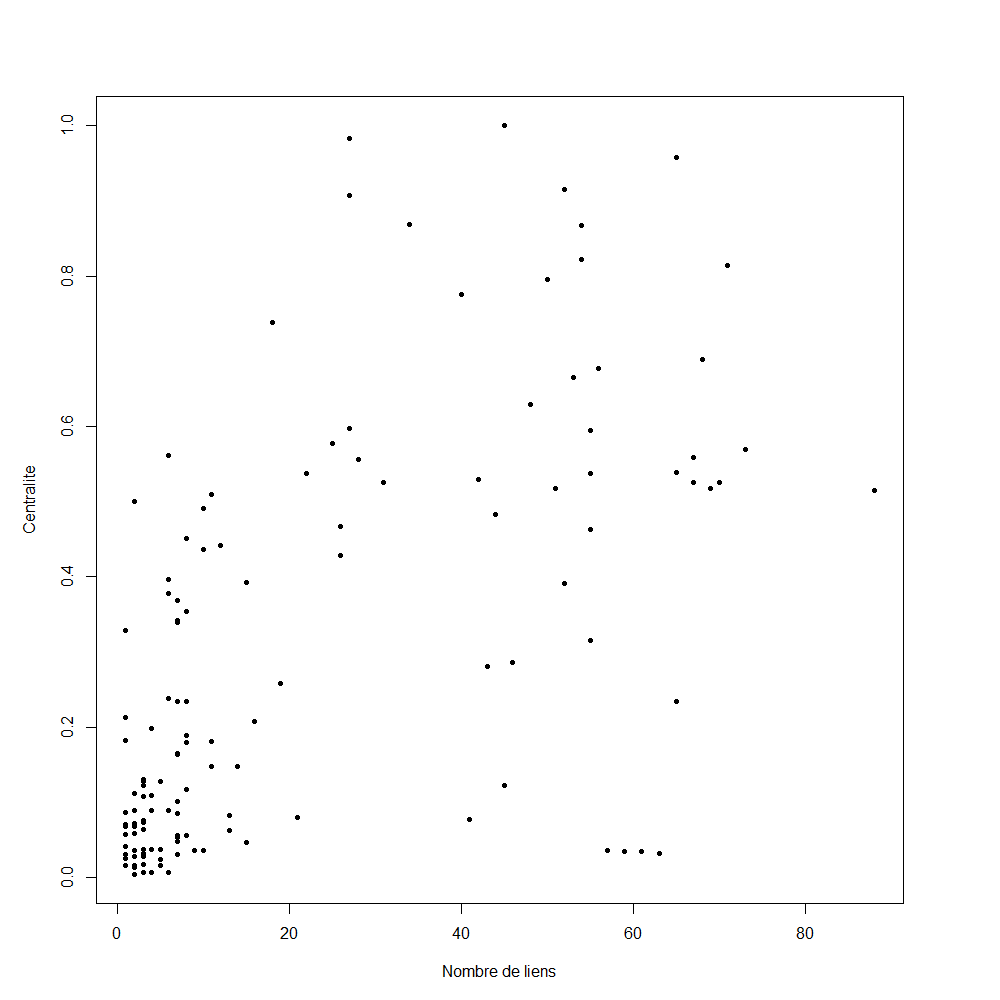
\includegraphics{images/ncollab_centralite.png}
\caption{Figure 2. Relation entre la centralité et le nombre de liens
des étudiants d'écologie à l'Université de Sherbrooke, 2023}
\end{figure}

La figure 2, de son côté nous informe de la corrélation entre le nombre
de liens ainsi que de la centralité entre tous les étudiants présents
dans l'étude. Il est possible de déterminer que la corrélation suit une
petite tendance positive dans notre cas. Il est important de noter que
les résultats de cette distribution sont significatifs étant donné que
le P \textless{} 0,05.

\begin{figure}
\centering
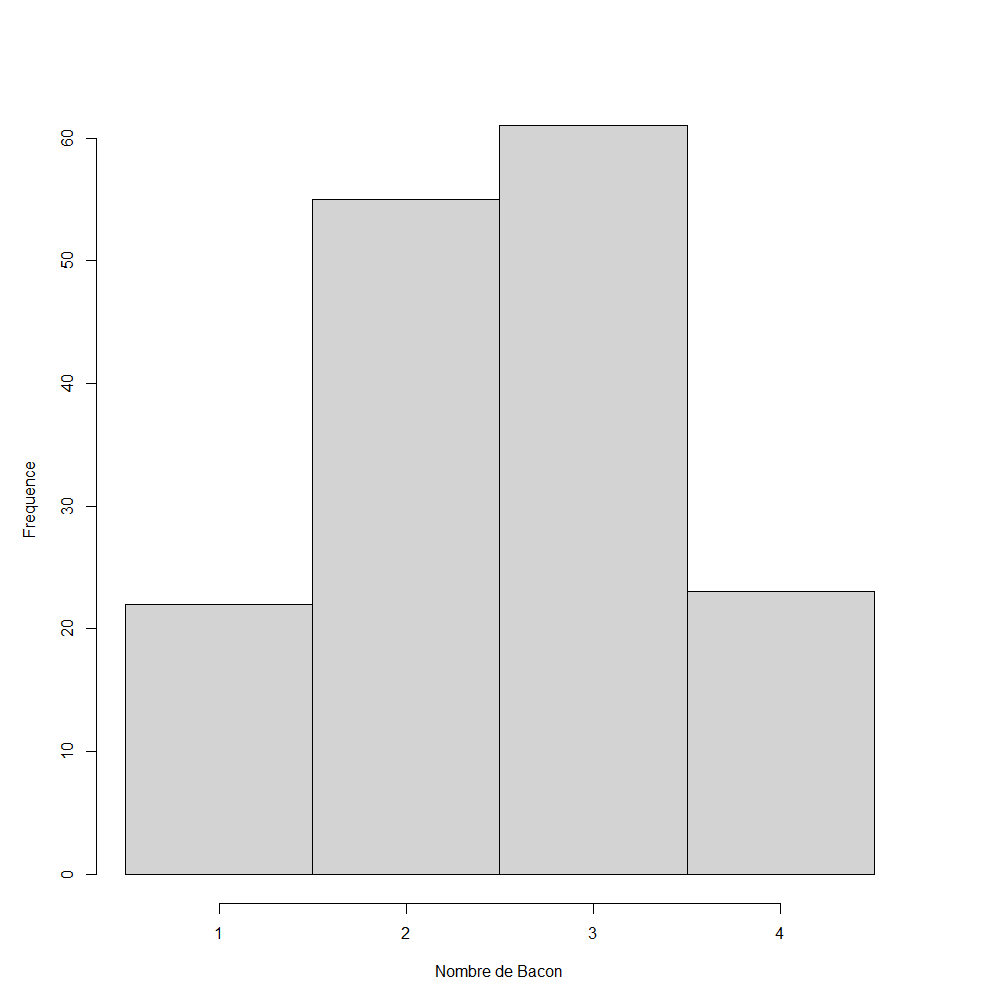
\includegraphics[width=5.20833in,height=\textheight]{images/b_number.png}
\caption{Figure 3. Degrés de séparation ``Bacon number'' avec Magalie
Bossé pour les étudiants d'écologie à l'Université de Sherbrooke, 2023}
\end{figure}

Au niveau de la figure 3, il est possible de voir le degré de séparation
entre les étudiants ainsi que l'étudiante Magalie Bossé. Donc il est
possible de conclure que la majorité des étudiants possède un degré de
séparation entre les valeurs 2 et 3, étant donné que ce sont les
colonnes les plus hautes du graphique.

\hypertarget{discussion}{%
\section{Discussion}\label{discussion}}

Pour commencer, si l'on regarde la figure 1, il est possible de voir que
ce type de réseau est bel et bien considéré comme étant un réseau petit
monde. En effet, comme il a été possible de constater, les connexions
entre les étudiants sont nombreuses et l'on peut affirmer que les
étudiants sont tous reliés. Comme démontrer dans une étude de
psychosociologie (Milgram {[}1967{]}), il est possible de relier deux
individus quelconques à travers de multiples connexions en se fixant un
nombre maximal de 6 degrés de séparation (1). L'expression 6 degrés de
séparation signifie qu'il va y avoir un maximum de 6 interactions entre
deux différents individus pour qu'ils soient reliés (1). On peut donc
conclure dans notre cas que cette règle s'applique si l'on regarde le
nombre de liens entre 2 étudiants étant extrêmement distancés.

La figure 2, de son côté, nous démontre le nombre de collaborations pour
chaque étudiant en fonction de leur centralité dans le réseau de
collaborations établi. La centralité ne mesure pas le nombre de liens,
mais plutôt à quel point le nœud occupe un certain type de position dans
le réseau de collaboration (3). Donc, on peut affirmer que la centralité
est plutôt associée à l'importance de la position d'un nœud. Si un nœud
se trouve à être le seul pont entre beaucoup d'individus, sa centralité
va donc se trouver beaucoup plus grande que le reste (3). Dans notre
étude, il est important de mentionner la centralité augmente lorsque le
nombre de liens augmente. Ce résultat concorde pleinement avec celui
relié à un réseau de type petit monde (1).

Du côté de la figure 3, il est possible de voir le nombre d'interactions
qui vont venir séparer notre étudiante de référence, Magalie Bossé, et
les autres étudiants présents dans le réseau de collaboration. Magalie
Bossé est l'étudiante choisie étant donné qu'elle possède le plus de
collaboration. Le nombre de bacon correspond au nombre d'interactions
entre un individu et l'individu de référence (2). Comme mentionné
précédemment, le nombre maximal de nœuds entre chaque individu est
établi à 6 (1). Par exemple, une activité exécutée dans le monde des
acteurs avec Kevin Bacon pour permettre de retracer le nombre de bacon
pour chaque acteur en référence à K. Bacon (2). Donc un acteur ayant
participé au même film que Kevin Bacon possède un nombre de 1. Dans
notre cas, les nombres oscillent entre 1 et 4 et la majorité des bacon
number se trouve à être 2 ou 3 (figure 3). Nos résultats concordent donc
parfaitement avec la littérature étant donné que le nombre maximal de
nœuds entre notre étudiant de référence et un autre étudiant est de 4.

\hypertarget{conclusion}{%
\section{Conclusion}\label{conclusion}}

Pour conclure, l'objectif principal qui consistait en la réalisation
d'un réseau de type petit monde pour les relations entre les étudiants
du cours de BIO500 de l'Université de Sherbrooke à l'hiver 2023 a été
réalisé. Par la suite, le bacon number de chaque individu a pu être
calculé en fonction d'un individu de référence pour voir si les bacon
number obtenus dépassaient le seuil de la littérature qui était de 6. Le
nombre maximal obtenu était de 4 donc cela concorde. Finalement, nous
avons pu déterminer la corrélation entre le nombre de liens ainsi que la
centralité de chaque étudiant à l'aide d'une représentation via un nuage
de points. De plus, il pourrait être intéressant d'effectuer un test de
centralité différent étant donné qu'il existe plusieurs centralités. Par
exemple, une centralité axée sur la proximité des nœuds permettrait de
trouver une centralité axée sur la personne qui est le plus près de tous
les autres individus du réseau (3).

\newpage

\hypertarget{bibliographie}{%
\section*{Bibliographie}\label{bibliographie}}
\addcontentsline{toc}{section}{Bibliographie}

\end{document}
